\section{Experiments}\label{sec:exp}
We present experimental results on three main-stream segmentation tasks: semantic segmentation, semi-supervised semantic segmentation, and domain adaptive semantic segmentation.
%
Besides, we present comparisons with previous works towards class-imbalanced problems.
%
The mean of Intersection over Union (mIoU) is adopted as the metric to evaluate all the results.


\subsection{Towards Fully Supervised Setting}\label{sec:fully_super}
\noindent\textbf{Datasets.} We used the typical long-tailed dataset: Cityscapes~\cite{cityscapes}.
%
Cityscapes is a driving dataset for semantic segmentation, which consists of 5000 high-resolution images for training and 500 images for validation.
%
We first resize the training images into a resolution of $2048\times1024$, then crop them into $512\times1024$.
%

\noindent\textbf{Implementation details.} 
We used the mmsegmentation codebase~\cite{mmseg2020} and trained all the models with 8 Tesla V100 GPUs.
%
To validate the proposed method \method, we apply our method \method to various state-of-the-art semantic segmentation models including ResNet~\cite{he2016deep}, Swin-Transformer~\cite{liu2021swin}, Mix-Transformer~\cite{xie2021segformer}, ViT~\cite{dosovitskiy2020image} based encoder with OCRHead~\cite{yuan2020object}, K-NeT~\cite{zhang2021k}, PSPHead~\cite{pspnet}, SegformerHead~\cite{xie2021segformer}, UperHead~\cite{xiao2018unified} based decoders respectively.
%
The batch size is set to 16 for all models.
%
The training iterations are $160k$ for MiT-b0 + SegformerHead, $80k$ for Swin-T + K-Net and Vit-B16 + UperHead, $40k$ for all the other models.
%
We use AdamW optimizer for three transformer-based models: Swin-T + K-Net, MiT-b0 + SegformerHead, and Vit-B16 + UperHead, with a learning rate of $6\times10^{-5}$, weight decay of $0.01$, a linear learning rate warmup with $1.5k$ iterations and linear decay afterwards.
%
For all of the other models, we use the same configuration: SGD optimizer with a learning rate of $0.01$, a weight decay of $5\times 10^{-4}$.


\noindent\textbf{Results.} 
Table \cref{tab:fully_supervised} summarizes the detailed comparison results across different architectures.
%
We observe that our method boosts all of these baseline models consistently.
%
Equipped with our method, these models gains $+0.72\%$, $+0.43\%$, $+0.55\%$, $+0.24\%$, $+0.47\%$, $+0.35\%$, $+1.20\%$ respectively without any additional model parameters.
%
The performance gains on various models with different network structures, including CNN-based and Transformer based models, indicate that our method is universal and can be generalized to various segmentation models.
%
To verify the effectiveness of \method towards long-tail data, we compute mIoU on \textbf{9} tail categories: \textit{Wall}, \textit{T.light}, \textit{Sign}, \textit{Rider}, \textit{Truck}, \textit{Bus}, \textit{Train}, \textit{M.bike}, \textit{Bike}.
%
The ``mIoU (tail)'' column demonstrates that the \method indeed boosts the performance of these tail categories by a large margin.

\subsection{Towards Semi-Supervised Setting}\label{sec:semi_exp}
\noindent\textbf{Datasets.} Semi-Supervised semantic segmentation aims to learn a model with only a few labeled samples.
%
Two typical benchmark datasets are usually used for validation: PASCAL VOC 2012\cite{voc} and Cityscapes\cite{cityscapes}.
%
PASCAL VOC 2012 is a class-balanced and simpler dataset.
%
Therefore, we mainly conduct experimental verification on Cityscapes.
%
We follow the commonly used $1/16$, $1/8$, $1/4$ and $1/2$ partition protocols, that is, only the corresponding fraction number have labels, and the rest of the images are considered unlabeled.
%
It is worth mentioning that our method adopts the generally used sliding window evaluation when evaluating.
%

%
\noindent\textbf{Implementation details.} The classical Self-Training~\cite{amini2022self} without any other tricks as the baseline due to its simplicity and to be consistent with our proposed method.
%
The core of semi-supervised segmentation methods is the training strategy, not the network structure.
%
So we use ResNet-101~\cite{he2016deep} as the backbone and DeepLabv3+~\cite{deeplab} as the decoder.
%
We use stochastic gradient descent (SGD) optimizer with an initial learning rate of $0.01$, and weight decay as $0.0005$.
%
The momentum coefficient $\mu$ for Teacher model~\cite{tarvainen2017mean} updating is set to $0.999$.
%
The crop size is set as $769\times 769$ and batchsize is set as 16.

%
\noindent\textbf{Results.} With our proposed \method, \cref{tab:semi} demonstrates that naive self-training framework achieves consistent performance gains over the naive self-training baseline by $+1.05\%$, $+1.26\%$, $+1.49\%$, $+0.99\%$ under $1/16$, $1/8$, $1/4$ and $1/2$ partition protocols.
%
To verify the effectiveness of \method towards long-tail data in semi-supervised segmentation task, we also list the ``mIoU(tail)'' column as the \cref{sec:fully_super}.
%
This demonstrates that the \method indeed improves the performance of the tail categories.
\begin{table}[t]
\centering
\caption{%
Experiments across architectures for fully semantic segmentation tasks on \textbf{Cityscapes} \textit{validation} set.
%
The green arrows indicate the relative improvement in performance.
}
\label{tab:fully_supervised}
\vspace{-8pt}
\setlength{\tabcolsep}{3pt}
\scalebox{0.85}{
\begin{tabular}{ll|ll}
\toprule
Backbone & Decoder & mIoU & mIoU (tail) \\
\midrule
\multirow{2}{*}{HRNet-18~\cite{sun2019deep}} & OCRHead~\cite{yuan2020object} & 79.22 & 63.51\\
&\textbf{ + \method} & \textbf{79.94\up{0.72}} & \textbf{66.70\up{3.19}}\\
\midrule 
\multirow{2}{*}{ResNet50~\cite{deeplab}} &UperHead~\cite{xiao2018unified} &78.28&62.56 \\
&\textbf{ + \method} & \textbf{78.63\up{0.35}}& \textbf{64.57\up{2.01}}\\
\midrule
\multirow{2}{*}{ResNet50~\cite{he2016deep}} & PSPHead~\cite{pspnet}& 77.98 & 61.96 \\
 &\textbf{ + \method} & \textbf{78.53\up{0.55}}&\textbf{63.34\up{1.38}}\\
\midrule
\multirow{2}{*}{ResNet101~\cite{he2016deep}} &UperHead~\cite{xiao2018unified} &79.41 &64.68 \\
&\textbf{ + \method} & \textbf{79.88\up{0.47}}&\textbf{66.29\up{1.61}}\\

\midrule
\multirow{2}{*}{MiT-b0~\cite{xie2021segformer}}& SegformerHead~\cite{xie2021segformer} & 76.85&67.58 \\
&\textbf{ + \method} & \textbf{77.09\up{0.24}}&\textbf{68.91\up{1.33}}\\
\midrule
\multirow{2}{*}{Swin-T~\cite{liu2021swin}} & K-NeT~\cite{zhang2021k} & 79.68& 71.70\\
&\textbf{ + \method} & \textbf{80.11\up{0.43}} & \textbf{72.94\up{1.24}}\\
\midrule
\multirow{2}{*}{Vit-B16~\cite{dosovitskiy2020image}}&UperHead~\cite{xiao2018unified}&76.48&68.25\\
&\textbf{ + \method} & \textbf{77.68\up{1.20}}&\textbf{70.63\up{2.38}}\\
\bottomrule
\end{tabular}}
%\vspace{-10pt}
\end{table}

% \begin{table}[t]
% \centering
% \caption{%
% Experiments on semi-supervise semantic segmentation tasks on \textbf{Cityscapes} \textit{validation} set. 
% %
% The green arrows indicate the relative improvement in performance.
% }
% \label{tab:semi}
% \vspace{-8pt}
% \setlength{\tabcolsep}{4pt}

% \begin{tabular}{cccc}
% \toprule
% 1/16 (186) & 1/8 (372)& 1/4 (744) & 1/2 (1488) \\
% \midrule
% \multicolumn{4}{c}{\textit{Self-Training}} \\
% 68.21 & 72.01 & 74.03 &77.99 \\
% \midrule
% \multicolumn{4}{c}{\textit{Self-Training + \method}} \\
% \textbf{69.26\up{1.05}} &\textbf{73.27\up{1.26}} &\textbf{75.52\up{1.49}} & \textbf{78.98\up{0.99}} \\


% \bottomrule
% \end{tabular}
% \vspace{-5pt}
% \end{table}

\begin{table}[t]
\centering
\caption{%
Experiments on semi-supervised semantic segmentation tasks on \textbf{Cityscapes} \textit{validation} set. 
%
The green arrows indicate the relative improvement in performance.
}
\label{tab:semi}
\vspace{-8pt}
\setlength{\tabcolsep}{10pt}
\scalebox{0.85}{
\begin{tabular}{ll|ll}
\toprule
Partition & Method & mIoU& mIoU (tail)  \\
\midrule
\multirow{2}{*}{1/16 (186)} & Self-Training & 68.21 & 53.09   \\
 &\textbf{+\method} &\textbf{69.26\up{1.05}} &\textbf{55.23\up{2.14}} \\
\midrule
\multirow{2}{*}{1/8 (372)} & Self-Training & 72.01 &58.74   \\
 &\textbf{+\method}&\textbf{73.27\up{1.26}} & \textbf{60.33\up{1.59}}  \\
\midrule
\multirow{2}{*}{1/4 (744)} & Self-Training & 74.03 &  61.76 \\
 &\textbf{+\method}& \textbf{75.52\up{1.49}} & \textbf{63.51\up{1.75}}  \\
\midrule
\multirow{2}{*}{1/2 (1488)} & Self-Training & 77.99 &  65.96 \\
 &\textbf{+\method}& \textbf{78.98\up{0.99}} & \textbf{67.24\up{1.28}}   \\

\bottomrule
\end{tabular}}
\vspace{-10pt}
\end{table}



\subsection{Towards UDA Setting}\label{exp:uda}


\begin{table*}[t]
\centering
\caption{%
Comparison with state-of-the-art alternatives on \textit{GTA5 $\to$ Cityscapes} benchmark. 
%
The results are averaged over 3 random seeds.
%
The top performance is highlighted in \textbf{bold} font.
%
\dag\ indicates that the corresponding framework uses a CNN-based structure.
%
\ddag\ indicates that the corresponding framework uses a Transformer-based structure.
}
\label{tab:domain_gta}
\vspace{-8pt}
\setlength{\tabcolsep}{2.5pt}
\scalebox{0.9}{
\begin{tabular}{l | ccccccccccccccccccc | c}
\toprule
Method &
\rotatebox{90}{Road} & \rotatebox{90}{S.walk} & \rotatebox{90}{Build.} & \rotatebox{90}{Wall} & \rotatebox{90}{Fence} & \rotatebox{90}{Pole} & \rotatebox{90}{T.light} & \rotatebox{90}{Sign} & \rotatebox{90}{Veget.} & \rotatebox{90}{Terrain} & \rotatebox{90}{Sky} & \rotatebox{90}{Person} & \rotatebox{90}{Rider} & \rotatebox{90}{Car} & \rotatebox{90}{Truck} & \rotatebox{90}{Bus} & \rotatebox{90}{Train} & \rotatebox{90}{M.bike} & \rotatebox{90}{Bike} & mIoU \\
\midrule
source only$^{\dag}$ & 70.2 & 14.6 & 71.3 & 24.1 & 15.3 & 25.5 & 32.1 & 13.5 & 82.9 & 25.1 & 78.0 & 56.2 & 33.3 & 76.3 & 26.6 & 29.8 & 12.3 & 28.5 & 18.0 & 38.6 \\
\midrule
DAFormer$^{\dag}$ & 94.6 & 66.5 & 87.9 & 39.5 & 33.7 & 38.5 & 49.6 & 60.0 &  88.0 & \textbf{46.6} & 88.3 & \textbf{69.6} & 44.4& \textbf{89.0}&46.8&\textbf{56.8}&0.0&17.8&44.3 & 55.9\\
%
DAFormer (\textit{w/} \method)& \textbf{94.9} & \textbf{68.2} & \textbf{88.8} & \textbf{40.9} & \textbf{37.1} & \textbf{42.6} & \textbf{52.1} & \textbf{62.1} & \textbf{88.3} & 43.3 & \textbf{89.3} & 68.6 & \textbf{44.5}&88.9&\textbf{56.0}&54.6&\textbf{3.8}&\textbf{38.6}&\textbf{58.3}&\textbf{59.0}\\
\midrule
DAFormer$^\ddag$
& 95.7 & 70.2    & \textbf{89.4}     & 53.5 & 48.1  & 49.6 & \textbf{55.8}  & 59.4 & \textbf{89.9}       & 47.9   & \textbf{92.5} & 72.2   & \textbf{44.7}  & \textbf{92.3} & 74.5  & \textbf{78.2} & 65.1   & 55.9      & 61.8 & 68.3 \\
%
DAFormer (\textit{w/} \method)
& \textbf{96.2}	&\textbf{73.1}&	89.3&	\textbf{53.6}&	\textbf{55.7}&	\textbf{50.9}&	55.7&	\textbf{61.1}&	89.7&	\textbf{52.4}&	92.3&	\textbf{74.7}&	43.5&	91.6&	\textbf{74.6}&	77.4&	\textbf{69.2}&	\textbf{58.9}&	\textbf{62.3}& \textbf{69.6}
 \\ 
%
\midrule
HRDA$^{\ddag}$& 96.4 & 74.4 & 91.0 & \textbf{61.6} & 51.5 & 57.1 & \textbf{63.9} & 69.3 & 91.3 & 48.4 & 94.2 & \textbf{79.0} & 52.9 & \textbf{93.9} & \textbf{84.1} & \textbf{85.7} & 75.9 & 63.9 & 67.5 & 73.8\\
%
HRDA (\textit{w/} \method)&\textbf{96.7} &\textbf{76.6} &\textbf{91.5} &61.2 &\textbf{56.9} &\textbf{59.4} &62.2 &\textbf{72.8} &\textbf{91.5} &\textbf{51.2} &\textbf{94.3} &77.5 &\textbf{54.7} &93.5 & 83.2 & 84.7 & \textbf{79.7} &\textbf{68.1} &\textbf{67.6}
&\textbf{74.9}
 \\ 
\bottomrule
\end{tabular}}
%\vspace{-5pt}
\end{table*}


\begin{table*}[t]
\centering
\caption{%
Comparison with state-of-the-art alternatives on \textit{SYNTHIA $\to$ Cityscapes} benchmark. 
%
The results are averaged over 3 random seeds.
%
The mIoU and the mIoU* indicate we compute mean IoU over 16 and 13 categories, respectively.
%
The top performance is highlighted in \textbf{bold} font.
%
\dag\ indicates that the corresponding framework uses a CNN-based structure.
%
\ddag\ indicates that the corresponding framework uses a Transformer-based structure.
}
\label{tab:domain_synthia}
\vspace{-8pt}
\setlength{\tabcolsep}{3.5pt}
\scalebox{0.9}{
\begin{tabular}{l | cccccccccccccccc | cc}
\toprule
Method &
\rotatebox{90}{Road} & \rotatebox{90}{S.walk} & \rotatebox{90}{Build.} & \rotatebox{90}{Wall*} & \rotatebox{90}{Fence*} & \rotatebox{90}{Pole*} & \rotatebox{90}{T.light} & \rotatebox{90}{Sign} & \rotatebox{90}{Veget.} & \rotatebox{90}{Sky} & \rotatebox{90}{Person} & \rotatebox{90}{Rider} & \rotatebox{90}{Car} & \rotatebox{90}{Bus} & \rotatebox{90}{M.bike} & \rotatebox{90}{Bike} & mIoU & mIoU* \\
\midrule
% \multicolumn{1}{l}{\textit{}} &
%  \multicolumn{15}{c}{DeepLab-V2~\cite{chen2017deeplab} with ResNet-101~\cite{he2016deep}} \\
% \midrule
source only$^{\dag}$ & 55.6 & 23.8 & 74.6 & 9.2 & 0.2 & 24.4 & 6.1 & 12.1 & 74.8 & 79.0 & 55.3 & 19.1 & 39.6 & 23.3 & 13.7 & 25.0 & 33.5 & 38.6 \\
\midrule
DAFormer$^\dag$  
&62.2 & 24.5 & 85.3 & 23.4 & 2.5 & 38.5 & 47.7 & \textbf{51.1} & 84.0 & 81.8 & 70.5 & \textbf{41.3} & 77.9 & 46.6  & 45.3 & 60.3 & 52.7 & 59.9
\\
%
DAFormer (\textit{w/} \method)  
&\textbf{70.4}	&\textbf{28.9}&	\textbf{89.2}&	\textbf{25.2}&	\textbf{19.9}&	\textbf{40.2}&	\textbf{55.2}&	50.3&	\textbf{86.9}&	\textbf{84.2}&	\textbf{76.4}&	40.5&	\textbf{79.6}&	\textbf{51.3}&	\textbf{49.2}&	\textbf{61.2}&	\textbf{56.8}& \textbf{63.3}

\\ 
\midrule
% \multicolumn{1}{l}{\textit{Transformer-based}} & \multicolumn{17}{c}{DAFormer~\cite{hoyer2022daformer} with MiT-B5~\cite{xie2021segformer}} \\
% \midrule
%
DAFormer$^\ddag$
& 84.5 & 40.7   & 88.4    & 41.5 & \textbf{6.5}   & 50.0 & 55.0  & 54.6 & 86.0 & 89.8 & 73.2 & \textbf{48.2}  & 87.2 & 53.2 & 53.9 & 61.7 & 60.9 & 67.4\\
%
DAFormer (\textit{w/} \method) &
\textbf{86.7}&	\textbf{44.9}&	\textbf{89.0}&	\textbf{43.2}&	6.4&	\textbf{52.1}&	\textbf{60.0}&	\textbf{54.9}&	\textbf{88.2}&	\textbf{91.3}&	\textbf{74.9}&	46.1	&\textbf{88.6}&	\textbf{55.6}&	\textbf{55.0}&	\textbf{62.3}&	\textbf{62.5}&\textbf{69.0}\\ 
%
\midrule
%
HRDA$^\ddag$
& 85.2 & 47.7 & 88.8 & 49.5 & 4.8 & \textbf{57.2} & 65.7 & 60.9 & 85.3 & 92.9 & \textbf{79.4} & 52.8 & 89.0 & \textbf{64.7} & 63.9 & 64.9 & 65.8 & 72.7 \\
%
HRDA (\textit{w/} \method)&
\textbf{87.6}&	\textbf{47.9}&	\textbf{90.5}&	\textbf{50.4}&	\textbf{6.9}&	57.1&	64.3&	\textbf{65.3}&	\textbf{86.9}&	\textbf{93.4}&	78.9&	\textbf{54.9}&	\textbf{89.1}&	62.9&	\textbf{65.2}&	\textbf{66.8}&	\textbf{66.8} & \textbf{73.4}
 \\ 
%
\bottomrule
\end{tabular}}
\vspace{-10pt}
\end{table*}



\noindent\textbf{Datasets.} Unsupervised Domain adaptive (UDA) semantic segmentation aims at transferring the knowledge from a source domain to a target domain.
%
The source domain is a labeled dataset obtained from the synthetic images and the target domain is an unlabeled real image dataset.
%
We use two synthetic datasets: GTA5~\cite{richter2016playing_GTA} and SYNTHIA~\cite{ros2016synthia} as source domains respectively and use real images from Cityscapes~\cite{cityscapes} as the target domain.
%
In other words, We conduct experiments on two dataset settings: \textit{GTA5 $\to$ Cityscapes} and \textit{SYNTHIA $\to$ Cityscapes}.
%
It is worth mentioning that in \textit{SYNTHIA $\to$ Cityscapes}, $16$ and $13$ of the $19$ classes of Cityscapes are used to calculate mIoU, following the common practice~\cite{hoyer2022daformer}

%
\noindent\textbf{Implementation details.} We use the recent state-of-the-art frameworks DAFormer~\cite{hoyer2022daformer} and HRDA~\cite{hoyer2022hrda} as the baseline.
%
In addition, since DAFormer~\cite{hoyer2022daformer} is a pure Transformer-based framework that integrates some effective training strategies, to verify our method, we also try to replace the model structure with ResNet101~\cite{he2016deep} + DeepLabV2~\cite{deeplab}.
%
This version of DAFormer based on the CNN structure also illustrates the generality of our method.
%
In all UDA segmenetation experiments, AdamW~\cite{dozat2016incorporating} optimizer is utilized with a learning rate of $6\times 10^{-5}$ for the encoder and $6\times 10^{-4}$ for the decoder.
%
This optimizer is set to be with a weight decay of $0.01$ along with a linear learning rate warmup with $1.5k$ iterations and linear decay afterward.
%
During training, for the DAFormer-based methods, per batch input is set to be of two $512\times 512$ random crops.
%
For HRDA~\cite{hoyer2022hrda}, whose main motivation considers the training image resolution, we adopt the settings consistent with the paper.
%



\noindent\textbf{Results.} \cref{tab:domain_gta} and \cref{tab:domain_synthia} both suggest that our proposed \method can consistently improve the performance of the UDA segmentation task.
%
Our \method advances the baseline frameworks DAFormer$^\dag$, DAFormer$^\ddag$, HRDA$^\ddag$ with $+3.1\%$, $+1.3\%$, $+1.1\%$ respectively on \textit{GTA5 $\to$ Cityscapes} benchmark.
%
\method also advances DAFormer$^\dag$, DAFormer$^\ddag$, HRDA$^\ddag$ with $+4.1\%$, $+1.6\%$, $+1.0\%$ on the mIoU evaluation of 16 categories and  with $+3.4\%$, $+1.6\%$, $+0.7\%$ on the mIoU evaluation of 13 categories respectively on \textit{SYNTHIA $\to$ Cityscapes} benchmark.
%
From the per-category results in \cref{tab:domain_synthia} and \cref{tab:domain_gta}, we can observe that the improvement of our method for the overall mIoU comes from the improvement of IoU of the tail categories.
%
We make this conclusion even more obvious by plotting the pixel-level category frequency versus performance improvement on tail categories in figure~\cref{fig:tail}.
%
Our \method achieves $+3.1\%$, $+14.3\%$, $+2.3\%$, $+4.7\%$, $+32.7\%$ and $+17.6\%$ boosts on ``wall'', ``truck'', ``traffic light'', ``trailer'', ``motorcycle'' and ``bicycle'', respectively, which happen to belong to the tail categories, indicating that our method optimizes the feature space of the tail category which leads to consistent performance improvements.
%

\begin{figure}[t]
    \centering
    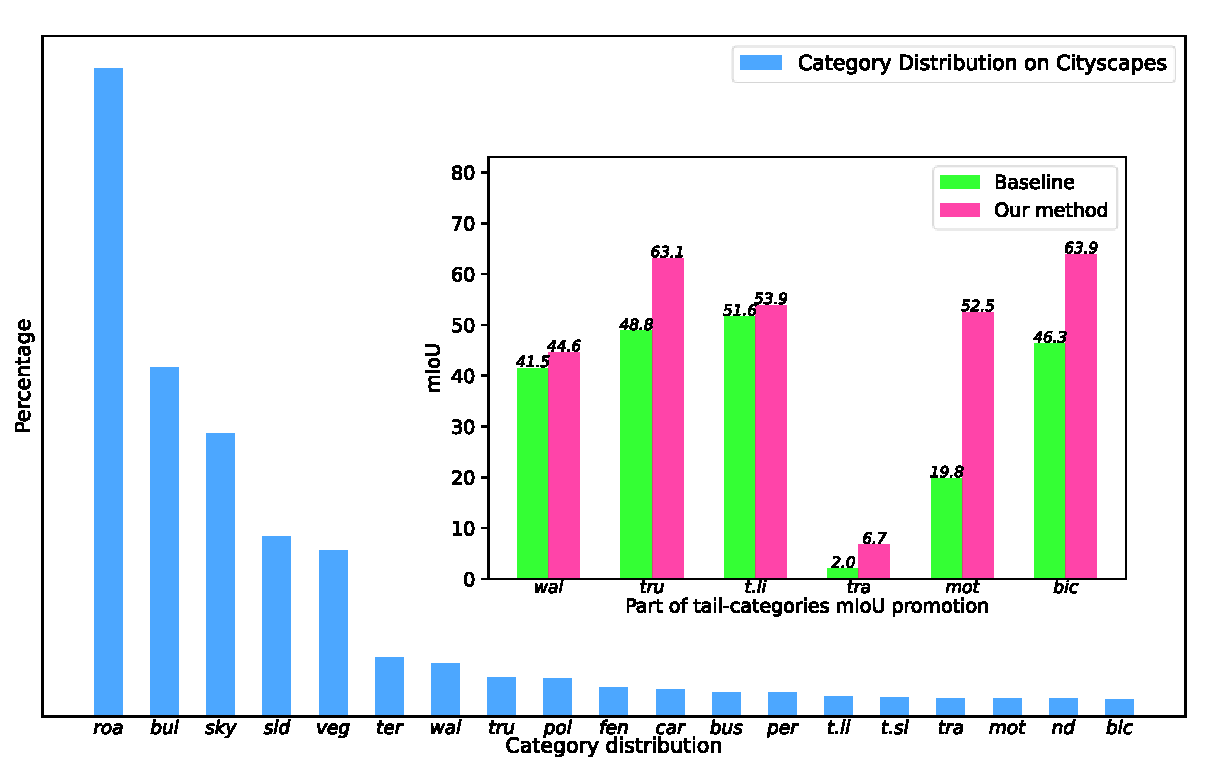
\includegraphics[width=1.0\linewidth]{figures/Exp_tail_categories.pdf}
    \vspace{-15pt}
    \caption{%
        %
        \textbf{Pixel-level category distribution versus performance improvement on multiple tail-categories.} This figure suggests that the performance improvement of our \method comes mainly from the tail category.
    }
    \label{fig:tail}
    \vspace{-18pt}
\end{figure}



\subsection{Comparisons with Long-tailed Methods}\label{sec:comparision}
\noindent \textbf{Implementation details.}  
%
For the fully-supervised setting, we implement Lovász-Softmax~\cite{berman2018lovasz} and Logit-Adjustment~\cite{menon2021long} loss on the ViT-B/16 + UperHead model.
%
For the semi-supervised setting, we implement \method and Logit-Adjustment~\cite{menon2021long} on the ResNet-50 + PSPNet model for a fair comparison with DARS~\cite{he2021re}.
%
For the UDA setting, we compare \method with naive resampling the input instances, CBST~\cite{li2022class}, CLAN~\cite{luo2019taking} and Logit-Adjustment~\cite{menon2021long} on \textit{GTA5 $\to$ Cityscapes}. 
%

%
\noindent \textbf{Results.}
% \todo{We will add more complete comparisons in the revision}.
We demonstrate more comparisons in \cref{tab:more_comparision}.
%
\method achieves the mIoU of $77.7\%$ on fully-supervised setting, $73.2\%$ on semi-supervised setting and $59.0\%$ on the domain adaptive setting.
%
\method also achieves the mIoU of $66.2\%$ on fully-supervised setting, $59.3\%$ on semi-supervised setting, and $45.7\%$ on the domain adaptive setting for the tail-categories.
%
The overall better performance suggests \method boosts the tail categories and outperforms other alternatives on different settings and benchmarks, which demonstrates its versatility and effectiveness.
%


\subsection{Ablation Studies}\label{sec:ablation}



\noindent \textbf{Exploration on the form of variations.} In \cref{tab:abla_1}, we explore the influence of different perturbation forms on the experimental results.
%
Results are obtained from the DAFormer$\dag$ framework on \textit{GTA5 $\to$ Cityscapes setting}.
%
``None-Variation'' denotes the pure baseline. 
%
``Gaussian'' variation parameters are illustrated in \cref{sec:method},
%
For the ``Uniform'' term, We sample uniformly in the interval $\left[0, 1\right]$, which brings in the baseline with a boost of $+2.3\%$.
%
For the ``Beta'' variation, we set the $\alpha=0.5$ and $\beta=0.5$, which advances the baseline by $+2.0\%$.
%
For the ``Exponential'' variation, we set the $\lambda=1$, which surpasses the baseline by $+2.6\%$ 
%
In order to ensure that the size of the perturbation is within a reasonable range, we clip all perturbations to the $\left[0, 1\right]$ interval.
%
We empirically find that the ``Gaussian'' variation term outperforms all the other alternatives with a mIoU of $59.0\%$, while all the other variations advance the baseline.
%
These suggest that various variations can improve the performance of the task, and the key to the improvement lies in the coefficients related to the category frequency rather than in the form of variation.
%
This is more in line with our intuition.
%
If the parameters of other variations are finetuned, better results may be obtained.
%


\noindent \textbf{Exploration on the variance $\sigma$.} As the only hyper-parameter needs to be carefully tuned, we ablate $\sigma$ for potential generalized usage extended to other tasks. 
%
\cref{tab:ablation_k} gives experimental results on the influence of different $\sigma$ with DAFormer $\dag$ under two different adaptation settings: \textit{GTA5 $\to$ Cityscapes} and \textit{SYNTHIA $\to$ Cityscapes}. 
%
\method advances the baseline most by $+3.1\%$ when $\sigma=6$ for \textit{GTA5 $\to$ Cityscapes} and  by $+4.1\%$ when $\sigma=4$ for \textit{SYNTHIA $\to$ Cityscapes}.
%
Although the different choices of $\sigma$ affect the final performance, these gaps are quite trivial(the discrepancy between the maximum and minimum mIoU is within $+1\%$), which demonstrates that our \method is robust to hyper-parameter choices to some extent and indicates its good scalability.


\begin{table}[t]
    \setlength{\tabcolsep}{5pt}
    \centering
    \caption{%
            More comparisons with other long-tailed baselines on different semantic segmentation tasks. 
            %
            ``RS'' and ``RW'' denotes the naive resample and reweight trick respectively.
            %
            %
            $^{\ast}$ means the results come from our implementation.
            %
            $^{\circ}$ means the results come from the original papers.
    }
    \label{tab:more_comparision}
    \vspace{-5pt}
    \scalebox{0.8}{
    \begin{tabular}{l|llllll}
        \toprule
    Supervision&\multicolumn{3}{c}{Fully} & \multicolumn{3}{|c}{Semi}  \\
       \midrule
Method & LA$^{\ast}$ &Lovász$^{\ast}$ & \method &\multicolumn{1}{|l}{LA$^{\ast}$}&DARS$^{\circ}$ & \method  \\
    \midrule
    mIoU&75.9 &76.6 & \textbf{77.7} & \multicolumn{1}{|l}{69.3} &72.8 &\textbf{73.2} \\
 mIoU (tail)&62.4  & 63.9 & \textbf{66.2} & \multicolumn{1}{|l}{55.7} & 58.4&\textbf{59.3}  \\
   \midrule
   Supervision&\multicolumn{6}{c}{Domain Adaptive}\\
   \midrule
   Method  &RS &RW &CLAN$^{\circ}$ & CBST$^{\circ}$ & LA$^{\ast}$ & \method \\
   \midrule
    mIoU& 56.2& 56.4&43.2 &45.9 &56.5 & \textbf{59.0} \\
     mIoU (tail)&40.5  &40.8  & 25.9 &28.5 &41.9 &\textbf{45.7} \\
%    mIoU(tail)& & 28.5 & 41.9 & \textbf{45.7} \\
        % U$^2$PL & 
        % \textbf{74.90} \scriptsize{(\textcolor{blue}{$+$0.45})} & \textbf{76.48} \scriptsize{(\textcolor{blue}{$+$0.93})} & \textbf{78.51} \scriptsize{(\textcolor{blue}{$+$1.03})} & \textbf{79.12} \scriptsize{(\textcolor{blue}{$+$0.11})} \\
        \bottomrule
    \end{tabular}
    }
    \vspace{-5pt}
\end{table}


\begin{table}[t]
\centering
\caption{%
\textbf{Ablation study on various types of variations.} ``None-Variation'' denotes the DAFormer$\dag$ baseline.
%
The green arrows indicate the relative improvement in performance.
}
\label{tab:abla_1}
\vspace{-5pt}
\setlength{\tabcolsep}{22pt}
\scalebox{1}{
\begin{tabular}{l | c  c}
\toprule
{Variation}&\multicolumn{2}{c}{mIoU} \\
\midrule
None-Variation & 55.9 &\\
Gaussian& \textbf{59.0}&\textbf{\up{3.1}} \\
Uniform & 58.2&\textbf{\up{2.3}}\\
Beta & 57.9&\textbf{\up{2.0}}\\
Exponential & 58.5&\textbf{\up{2.6}} \\

\bottomrule
\end{tabular}}
\vspace{-5pt}
\end{table}


\begin{table}[t]
\centering
\caption{%
%
\textbf{Ablation study on the variance $\sigma$ in \cref{eq:balancing},}
%
which determines the overall magnitude of the variation.
}
\setlength{\tabcolsep}{10pt}
\label{tab:ablation_k}
\vspace{-5pt}
\setlength{\tabcolsep}{9pt}
\begin{tabular}{cccccc}
\toprule
Baseline    &     3& 4 & 5 & 6 & 7   \\
\midrule
\multicolumn{6}{c}{\textit{GTA5 $\to$ Cityscapes}}
\\
55.9  & 58.0 &    58.8   &        58.2   &         \textbf{59.0}   &  58.7          \\
\midrule
\multicolumn{6}{c}{\textit{SYNTHIA $\to$ Cityscapes}} \\
52.7  &56.5  &   \textbf{56.8}    &   55.9        & 56.3           &   56.1         \\
\bottomrule
\end{tabular}
\vspace{-5pt}
\end{table}


%
\begin{table}[t]
\centering
\caption{%
%
\textbf{Ablation study on the components of \method.} 
%
We ablate two components in \cref{eq:balancing}.
%
``\textit{w/o} variation'' indicates removing the $|\delta(\sigma)|$ term.
%
``\textit{w/o} variation'' indicates removing the pixel-level category frequency term.
}
\setlength{\tabcolsep}{10pt}
\label{tab:ablation_components}
\vspace{-5pt}
\begin{tabular}{cccc}
\toprule
 Baseline & \textit{w/o} variation & \textit{w/o} balance& \method   \\
\midrule
\multicolumn{4}{c}{\textit{GTA5 $\to$ Cityscapes}} \\
 55.9 &   56.5      &    56.8 &    \textbf{59.0}          \\
\midrule
\multicolumn{4}{c}{\textit{SYNTHIA $\to$ Cityscapes}} \\
 52.7 &   53.9    &  54.5         &     \textbf{56.8}    \\
  
\bottomrule
\end{tabular}
\vspace{-10pt}
\end{table}

\begin{figure*}[t]
    \centering
    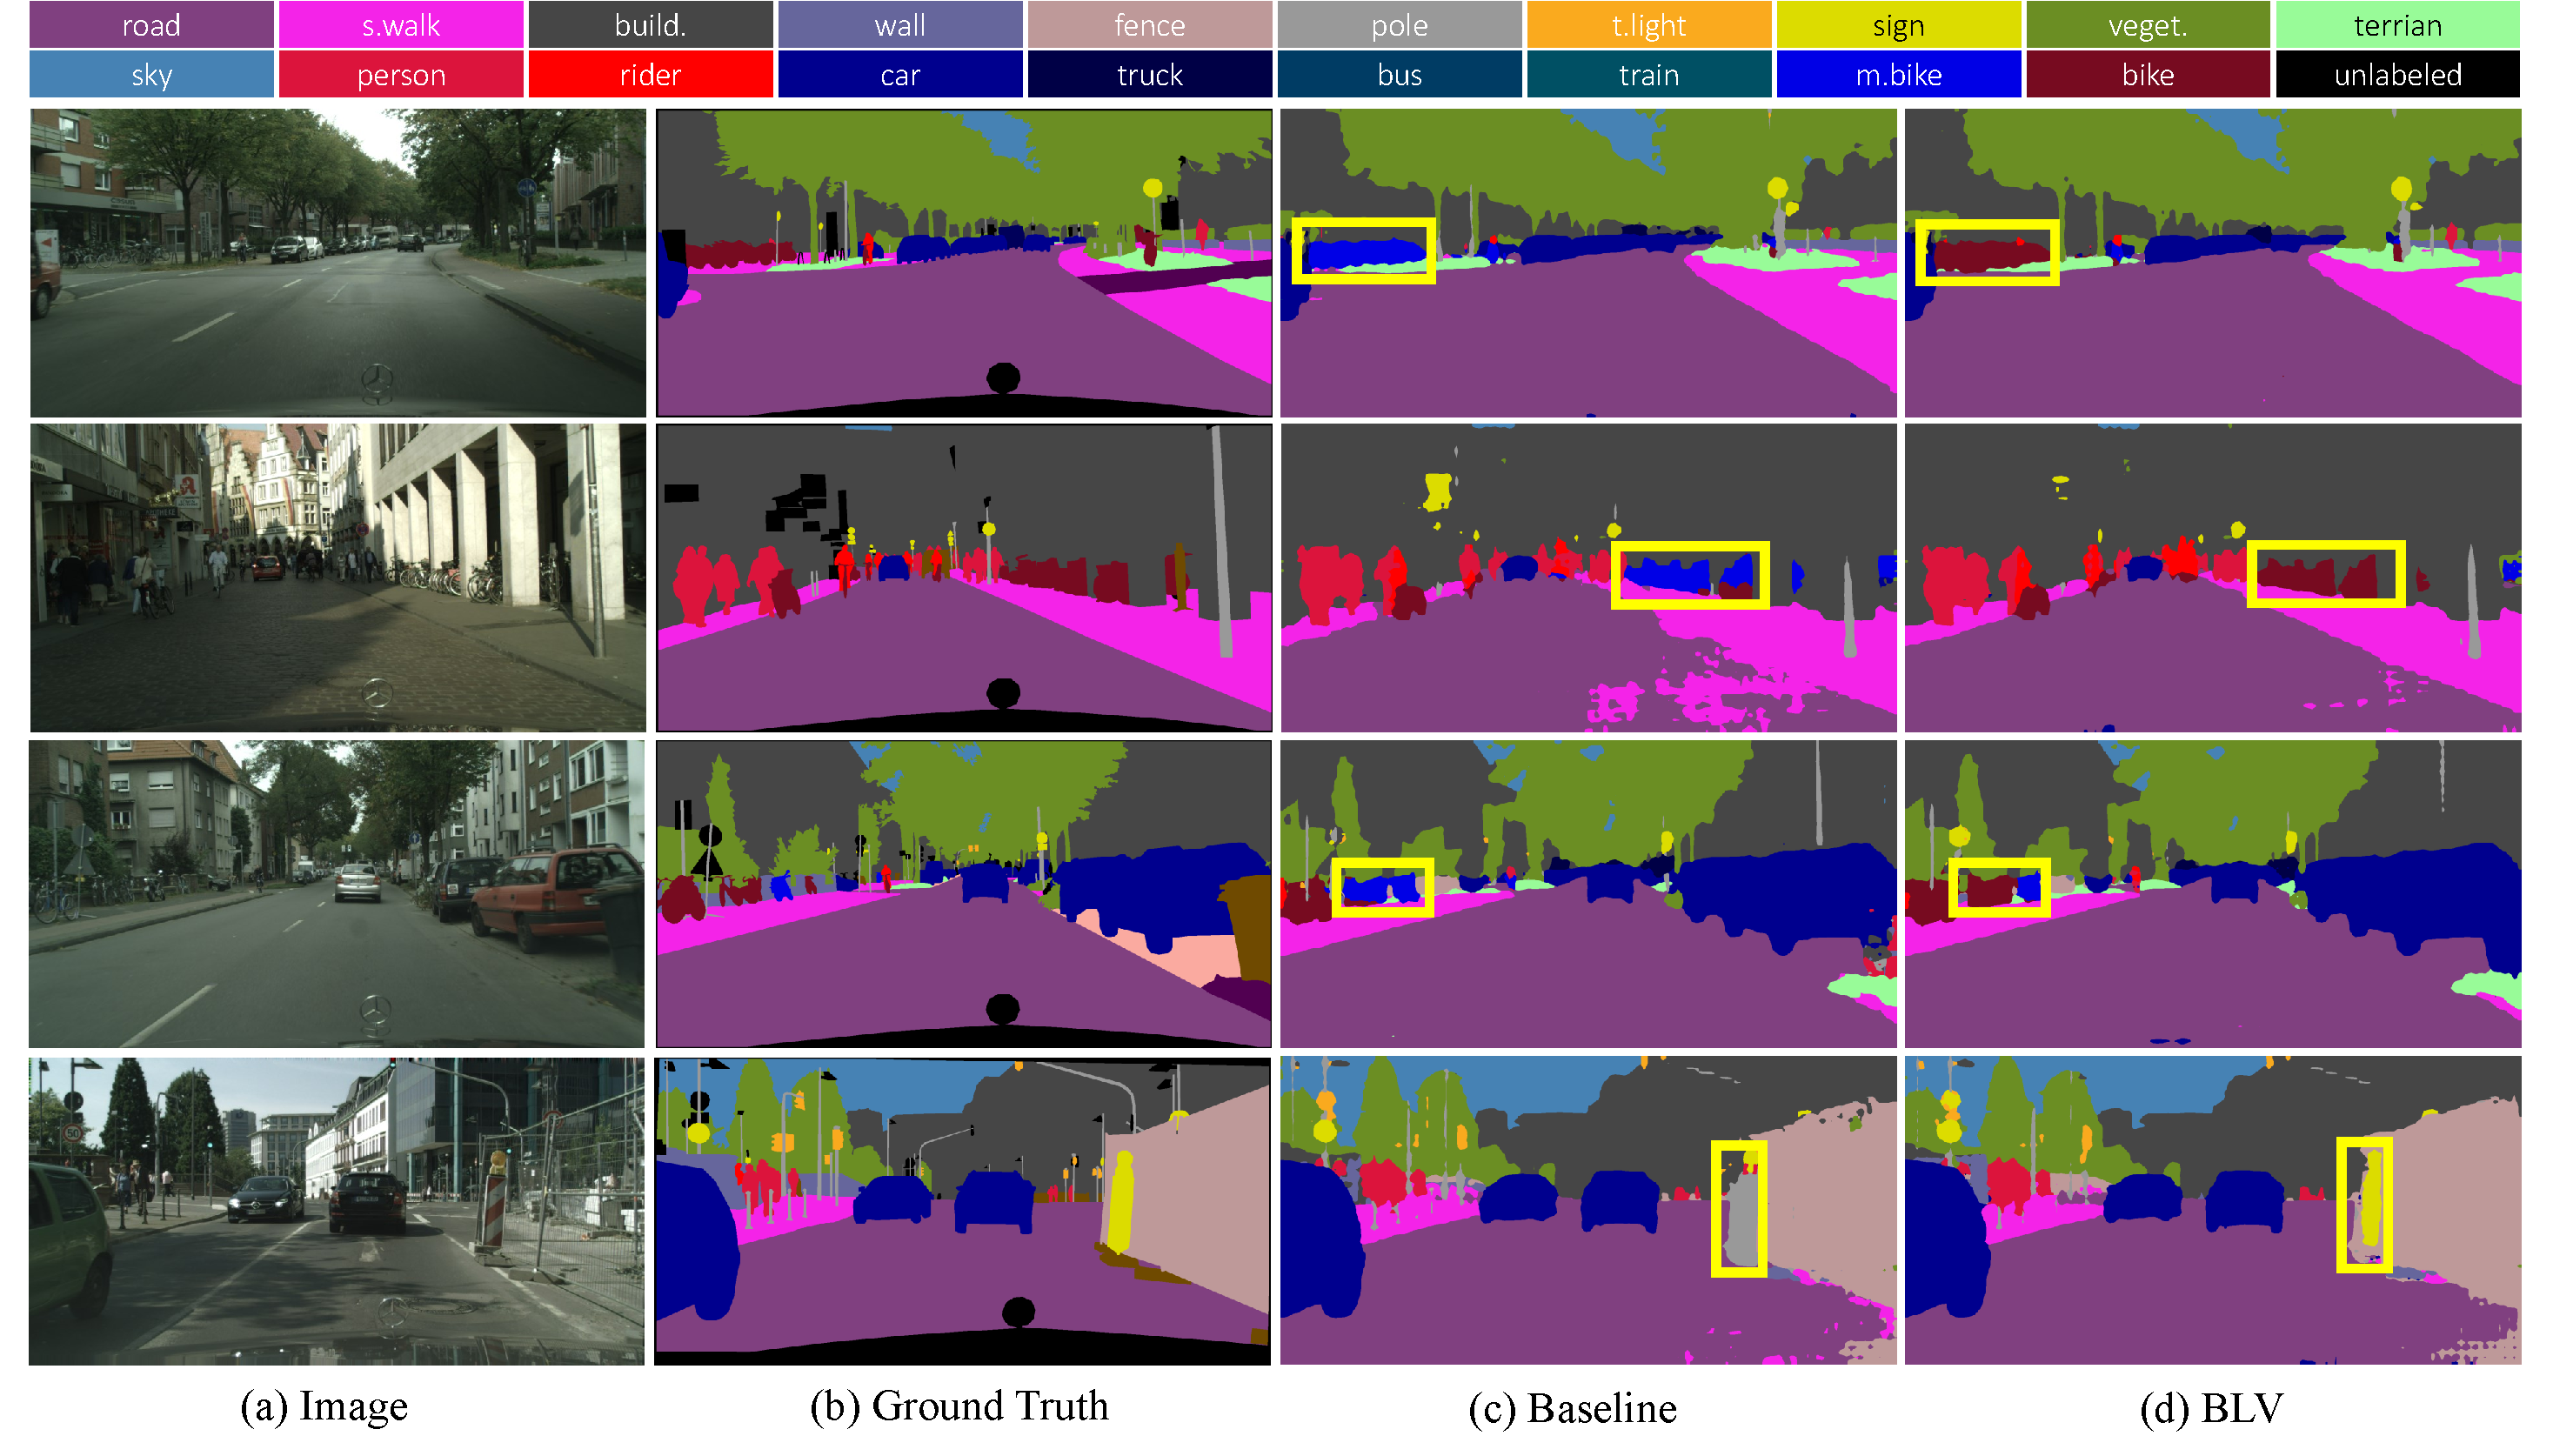
\includegraphics[width=1\textwidth]{figures/vis.pdf}
     \vspace{-18pt}
    \caption{%
    \textbf{Qualitative results on Cityscapes val set}.
    %
    Baseline and BLV are trained on \textit{GTA5$\to$ Cityscapes} benchmark of unsupervised domain adaptive semantic segmentation task.
    %
    (a) Input images. 
    %
    (b) Ground truth annotations for the corresponding images.
    %
    (c) Result of the DAFormer baseline.
    %
    (d) Result of our method (DAFormer + BLV).
    Yellow rectangles highlight the promotion of segmentation results by our method on tail categories.
    }
    \label{fig:vis}
    \vspace{-10pt}
\end{figure*}

\noindent \textbf{Exploration on components of \method.} Corresponding results are demonstrated in \cref{tab:ablation_components}.
%
``$\textit{w/o}$ variation'' denotes our \method without adding the variation in \cref{sec:method} rather a constant value adjustment for each category.
%
``$\textit{w/o}$ balance'' denotes our \method without adding categorical balance coefficient in \cref{sec:method} rather a fixed-scale adjustment for each category.
%
\cref{tab:ablation_components} demonstrates that either the ``$\textit{w/o}$ variation'' or ``$\textit{w/o}$ balance'' can boost the baseline non-trivially on both the \textit{GTA5 $\to$ Cityscapes} by $+0.6\%$, $+0.9\%$ and the \textit{SYNTHIA $\to$ Cityscapes} settings by $+1.2\%$, $+1.8\%$, although not as significant as our \method.
%
This suggests two conclusions: 
% 
1) Adding category-agnostic consistent variation to logits can indeed optimize the representation space to a certain extent, but it cannot completely solve the adverse effects of long-tailed data.
%
2) Adding static category-related adjustments can also alleviate this problem, but this cannot enrich training instances thus leading to potential overfitting problems while the variation term of \method can be used to avoid this problem efficiently.
%
This ablation experiment demonstrates the necessity of all components of our proposed \method.



%

% \begin{table}[t]
% \centering
% \caption{%
% %
% \textbf{Ablation study on other long-tailed alternative techniques of \method.}
% %
% ``Resample'' refers to balancing the number of categorical training instances.
% %
% ``Reweight'' refers to adding weights to the loss function that are inversely proportional to the category frequency.
% }
% \setlength{\tabcolsep}{13pt}
% \label{tab:ablation_others}
% \vspace{-8pt}
% \begin{tabular}{cccc}
% \toprule
%  Baseline &  Resample & Reweight & \method   \\
% \midrule
% \multicolumn{4}{c}{\textit{GTA5 $\to$ Cityscapes}} \\
%  55.9 &   56.2     &56.4     &    \textbf{59.0}          \\
% \midrule
% \multicolumn{4}{c}{\textit{SYNTHIA $\to$ Cityscapes}} \\
%  52.7 &  53.2     & 52.9          &     \textbf{56.8}                 \\
% \bottomrule
% \end{tabular}
% \vspace{-10pt}
% \end{table}




% \noindent \textbf{Exploration on other long-tailed alternative techiniques of \method.} 
% "Resample" and "Reweight" are two common techniques to alleviate long-tailed training data issues.
% %
% "Resample" changes the relative number of training instances for each category during model training.
% %
% In \cref{tab:ablation_others}, we resample the training data so that they achieve a consistent number of training instances for each category.
% %
% "Resample" boosts the baseline by $+0.3\%$ and $+0.5\%$ on both the \textit{GTA5 $\to$ Cityscapes} and the \textit{SYNTHIA $\to$ Cityscapes} respectively.
% %
% "Reweight" changes the weights of the loss function corresponding to the instances of each category, thus alleviating the effect of data imbalance on the gradient.
% %
% In \cref{tab:ablation_others}, we add a weight to each category that is inversely proportional to its number of instances in the total when calculating the loss.
% %
% "Reweight" advances the baseline by $+0.5\%$ and $+0.2\%$ on both the \textit{GTA5 $\to$ Cityscapes} and the \textit{SYNTHIA $\to$ Cityscapes} respectively.
% %
% \cref{tab:ablation_others} demonstrates that although both "Resample" and "Reweight" are valid for this task, our simple yet efficient method surpasses both the "Resample" and "Reweight" on both two settings.
%




\subsection{Visualization}
\cref{fig:vis} shows the result of our method on the Cityscapes val set.
%
With this visualization, we prove that overlaying our method to the baseline is effective in alleviating category confusion, so our method achieves better performance.
%
More details can be demonstrated by the yellow rectangle highlighting part in \cref{fig:vis}c and \cref{fig:vis}d. (\textit{i.e.} the pixel misclassified in the baseline are corrected by balancing logit variation.)
%